\chapter{最小作用量原理}

\problem{选取合适的广义坐标,求习题\ref{problem2-2}中系统的拉格朗日量和运动方程。}

\begin{solution}
	\begin{figure}[h]
		\centering
		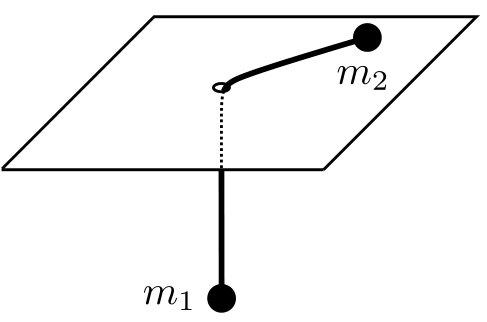
\includegraphics[width=0.3\textwidth]{content/Figures/2-2}
		\caption{ }
		\label{fig:4-1}
	\end{figure}
    原题如图\ref{fig:4-1}所示,选取\(m_2\)与小孔的距离\(r\)和\(m_2\)转动的角度\(\theta\)作为广义坐标。记绳长为\(l\),则\(m_1,m_2\)与小孔的距离分别可以表示为
    \begin{align*}
    	\begin{cases}
    		r_1=l-r\\
    		r_2=r
    	\end{cases}
    \end{align*}
    系统的动能可表示为
    \[T=\frac{1}{2}m_1 \dot{r}^2+\frac{1}{2}m_2(\dot{r}^2+r^2 \dot{\theta}^2)=\frac{1}{2}(m_1+m_2)\dot{r}^2+\frac{1}{2}m_2 r^2\dot{\theta}^2\]
    而势能则可计算为
    \[V=-m_1 g(l-r)\]
    于是Lagrangian为
    \[L=T-V=\frac{1}{2}(m_1+m_2)\dot{r}^2+\frac{1}{2}m_2 r^2\dot{\theta}^2+m_1 g(l-r)\]
    代入拉格朗日方程
    \[\frac{\partial L}{\partial r}-\frac{\dd }{\dd t}\frac{\partial L}{\partial \dot{r}}=0,\frac{\partial L}{\partial \theta}-\frac{\dd }{\dd t}\frac{\partial L}{\partial \dot{\theta}}=0\]
    得到运动方程为
    \begin{align*}
    	\begin{cases}
    		(m_1+m_2)\ddot{r}=m_2 r\dot{\theta}^2-m_1 g\\
    		\frac{\dd}{\dd t}(m_2 r^2 \dot{\theta})=0
    	\end{cases}
    \end{align*}
\end{solution}

\problem{选取合适的广义坐标,求习题\ref{problem2-3}中系统的拉格朗日量和运动方程。}
\begin{solution}
	\begin{figure}[h]
		\centering
		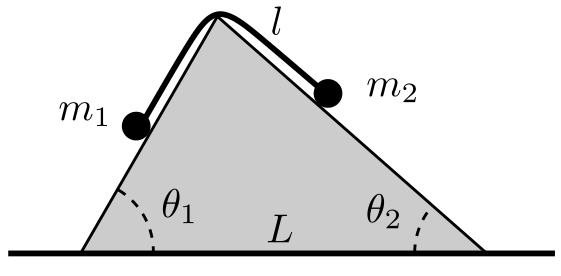
\includegraphics[width=0.3\textwidth]{content/Figures/2-3}
		\caption{ }
		\label{fig:4-2}
	\end{figure}
	原题如图\ref{fig:4-2}所示,无约束时的广义坐标为$\{x, r_1, r_2\}$,其中 $x$ 为楔块在水平面上的位置,$r_1$ 和 $r_2$ 分别是两个粒子到楔块尖端的距离,约束方程为
	\[\phi (r_1, r_2) = r_1 + r_2 - l = 0\]
	于是选取广义坐标\(r,x\),而\(r_1,r_2\)分别为
    \begin{align*}
		\begin{cases}
			r_1=r\\
			r_2=l-r
		\end{cases}
	\end{align*}
	为了方便,选取坐标原点到楔块最上方顶点的距离为\(x\),且两点等高,那么对两个块分别有
    \begin{align*}
		\begin{cases}
			x_1=x-r\cos{\theta_1},y_1=-r \sin{\theta_1}\\
			x_2=x+(l-r)\cos{\theta_2},y_2=-(l-r)\sin{\theta_2}
		\end{cases}
	\end{align*}
	系统的动能为
	\begin{align*}
		T&=\frac{1}{2}M\dot{x}^2 +\frac{1}{2}m_1(\dot x_1^2+\dot y_1^2)+\frac{1}{2}m_2(\dot x_2^2+\dot y_2^2)\\
		&=\frac{1}{2}M\dot{x}^2+\frac{1}{2} m_1 \left(\sin^2{\theta_1} \dot r^2+\left(\dot x-\cos{\theta_1} \dot r\right)^2\right)+\frac{1}{2} m_2 \left(\sin^2{\theta_2} \dot r^2+\left(\dot x-\cos{\theta_2} \dot r\right)^2\right)\\
		&=\frac{1}{2} \left((M+m_1+m_2) \dot x^2-2 (m_1 \cos{\theta_1}+m_2 \cos{\theta_2})\dot r \dot x +(m_1+m_2) \dot r^2\right)\\
		&=\frac{1}{2}(M+m_1+m_2) \dot x^2-(m_1 \cos{\theta_1}+m_2 \cos{\theta_2})\dot r \dot x +\frac{1}{2}(m_1+m_2) \dot r^2
	\end{align*}
	势能则为
	\[V=m_1 g y_1+m_2 g y_2=-m_1 g r\cos{\theta_1}-m_2 g(l-r)\cos{\theta_2}\]
	拉格朗日量则是
	\[L=T-V=\frac{1}{2}(M+m_1+m_2) \dot x^2-(m_1 \cos{\theta_1}+m_2 \cos{\theta_2})\dot r \dot x +\frac{1}{2}(m_1+m_2) \dot r^2+(m_1\cos{\theta_1}-m_2\cos{\theta_2})g r+m_2 g l \cos{\theta_2}\]
	代入拉格朗日方程
	\begin{align*}
		\frac{\partial L}{\partial x}-\frac{\dd}{\dd t}\frac{\partial L}{\partial \dot{x}}=0\\
		\frac{\partial L}{\partial r}-\frac{\dd}{\dd t}\frac{\partial L}{\partial \dot{r}}=0
	\end{align*}
	计算得到运动方程为
	\begin{align*}
		(m_1\cos{\theta_1}+m_2\cos{\theta_2}) \ddot{r}-(M+m_1+m_2)\ddot{x}=0\\
		-(m_1+m_2)\ddot{r}+(m_1\cos{\theta_1}+m_2\cos{\theta_2})\ddot{x}+(m_1\cos{\theta_1}-m_2\cos{\theta_2})g=0
	\end{align*}
\end{solution}


\problem{选取合适的广义坐标,求习题\ref{problem2-4}中系统的拉格朗日量和运动方程。}
\begin{solution}
    \begin{figure}[h]
    	\centering
    	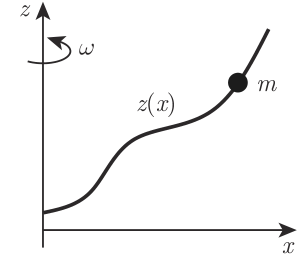
\includegraphics[width=0.2\textwidth]{content/Figures/2-4}
    	\caption{ }
    	\label{fig:4-3}
    \end{figure}
    原题如\ref{fig:4-3}所示,由于只有一个自由度,不妨选取\(x\)为广义坐标。在柱坐标系中,粒子坐标为
    \begin{align*}
    	\rho&=x\\
    	\theta&=\omega t\\
    	z&=z(x)
    \end{align*}
    其动能表达式为
    \[T=\frac{1}{2}m(\dot{\rho}^2+\rho^2 \dot{\theta}^2+\dot{z}^2)=\frac{1}{2}m (1+z'(x)^2)\dot{x}^2+\frac{1}{2}m\omega^2 x^2\]
    势能则为
    \[V=mgz=mg z(x)\]
    拉格朗日量为
    \[L=T-V=\frac{1}{2}m (1+z'(x)^2)\dot{x}^2+\frac{1}{2}m\omega^2 x^2-mg z(x)\]
    代入欧拉-拉格朗日方程
    \[\frac{\partial L}{\partial x}-\frac{\dd}{\dd t}\frac{\partial L}{\partial \dot{x}}=0\]
    得到运动方程为
    \[m\omega^2 x-mgz'(x)-\frac{\dd}{\dd t}\left[m(1+z'(x)^2)\dot{x}\right]=0\]
\end{solution}


\problem{如图\ref{fig:4-4}所示,长为\(l\)质量为\(m\)的匀质硬杆,一端置于地面,一端靠在墙角,杆始终处于竖直平面内。忽略摩擦,已知杆相对质心的转动惯量为\(I=\frac{1}{12}m l^2\)。选择合适的广义坐标,写出系统的拉格朗日量并求系统的运动方程。}
\begin{figure}[h]
	\centering
	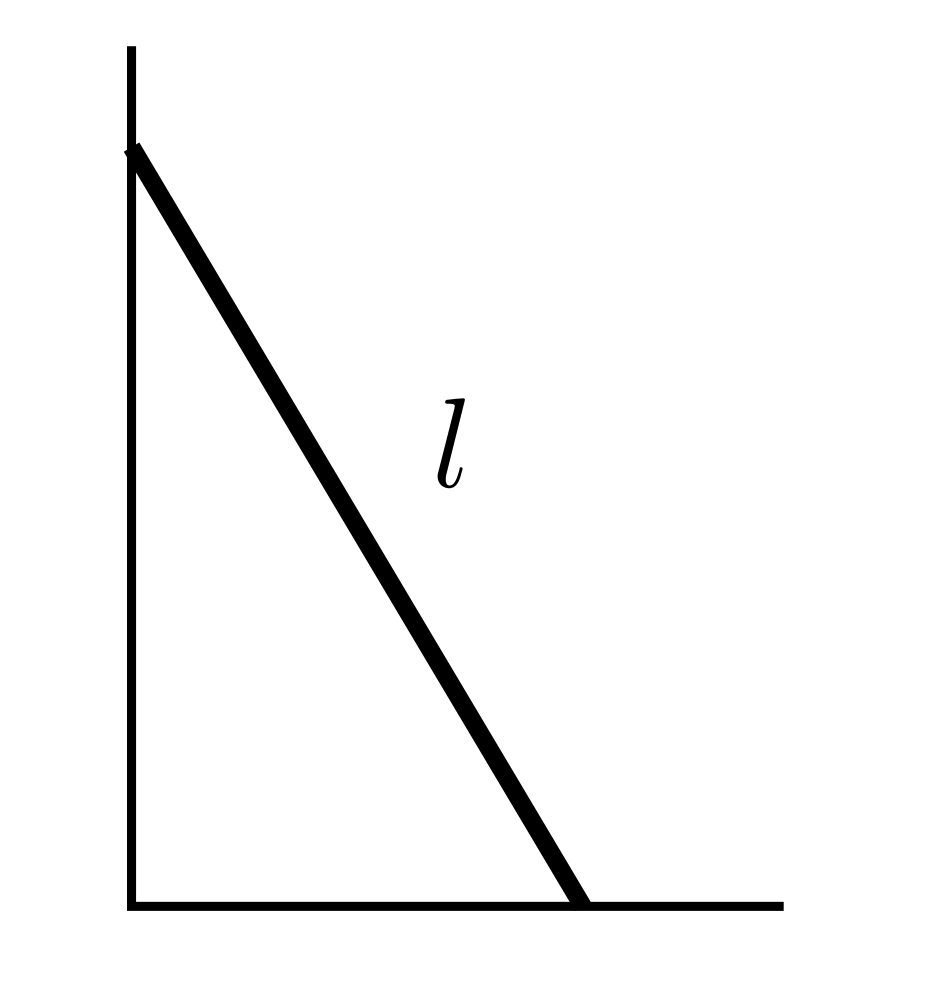
\includegraphics[width=0.2\textwidth]{content/Figures/4-4}
	\caption{ }
	\label{fig:4-4}
\end{figure}

\begin{solution}
    为方便,选取杆与墙的夹角\(\theta\)为广义坐标,那么杆的质心坐标为
    \begin{align*}
    	x_c&=\frac{l}{2}\sin{\theta}\\
    	y_c&=\frac{l}{2}\cos{\theta}
    \end{align*}
    计算出系统动能为
    \[T=\frac{1}{2}m(\dot{x_c}^2+\dot{y_c}^2)+\frac{1}{2}I\dot{\theta}^2=\frac{1}{6}ml^2\dot{\theta}^2\]
    而势能为
    \[V=mgy_c=mg\frac{l}{2}\cos{\theta}\]
    于是拉格朗日量为
    \[L=T-V=\frac{1}{6}ml^2\dot{\theta}^2-mg\frac{l}{2}\cos{\theta}\]
    代入欧拉-拉格朗日方程
    \[\frac{\partial L}{\partial \theta}-\frac{\dd}{\dd t}\frac{\partial L}{\partial \dot{\theta}}=0\]
    结果为
    \[mg\frac{l}{2}\sin{\theta}-\frac{1}{3}ml^2\ddot{\theta}=0\]
    整理为
    \[\ddot{\theta}=\frac{3g}{2l}\sin{\theta}\]
\end{solution}


\problem{如图\ref{fig:4-5}所示,半径为\(R\)的圆环固定于竖直平面内,两个质量为\(m\)的小球由自由长度为\(l\)的无质量弹簧连接,小球可沿圆环无摩擦滑动。选择合适的广义坐标,写出系统的拉格朗日量并求系统的运动方程。}
\begin{figure}[h]
	\centering
	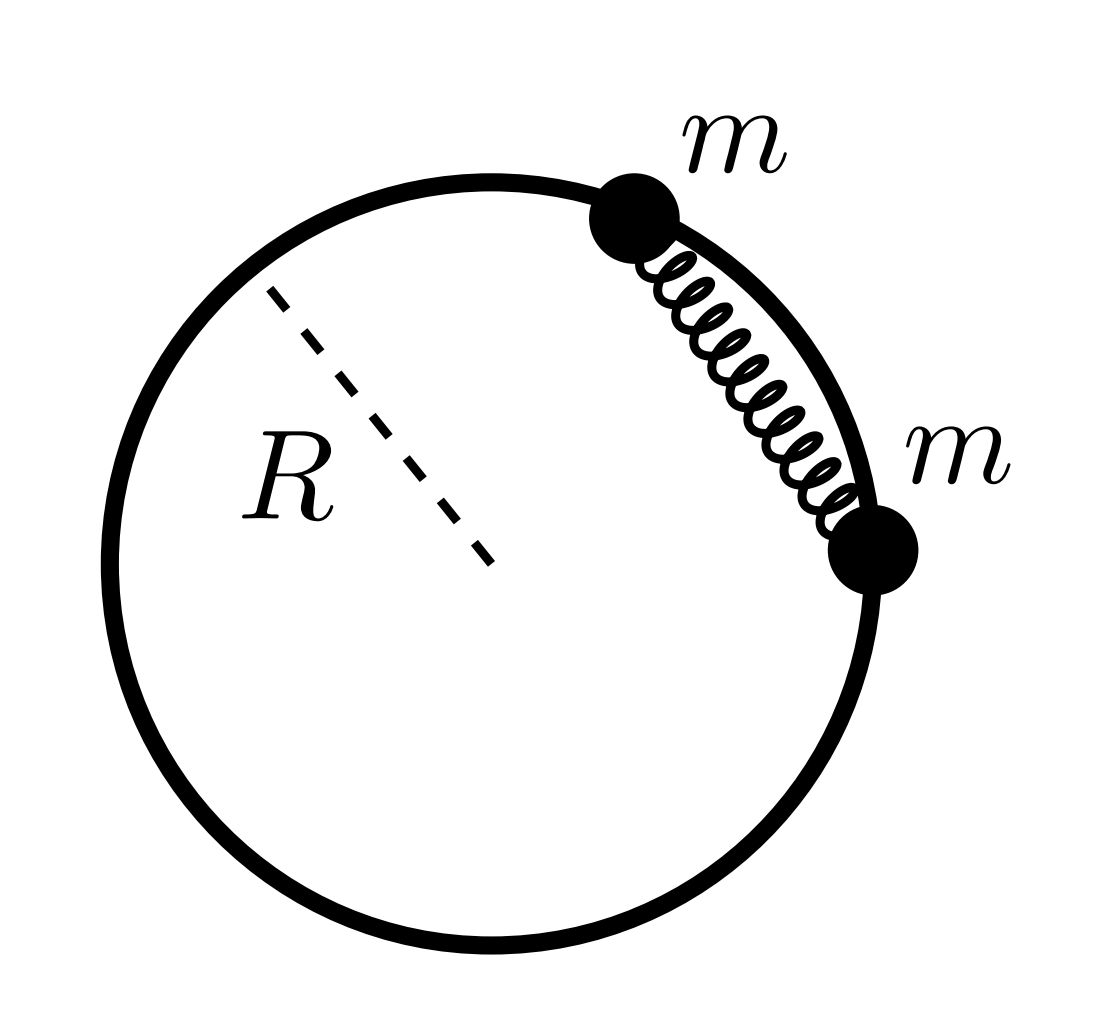
\includegraphics[width=0.2\textwidth]{content/Figures/4-5}
	\caption{ }
	\label{fig:4-5}
\end{figure}

\begin{solution}
    选两个小球相对参考线的转角\(\theta_1,\theta_2\)作为广义坐标。动能显然为
    \[T=\frac{1}{2}m_1 R^2 \dot{\theta}_1^2+\frac{1}{2}m_2 R^2 \dot{\theta}_2^2\]
    而势能则为
    \[V=\frac{1}{2}k (2R\sin{\frac{\theta_2-\theta_1}{2}}-l)^2\]
    拉格朗日量为
    \[L=T-V=\frac{1}{2}m_1 R^2 \dot{\theta}_1^2+\frac{1}{2}m_2 R^2 \dot{\theta}_2^2-\frac{1}{2}k (2R\sin{\frac{\theta_2-\theta_1}{2}}-l)^2\]
    代入欧拉-拉格朗日方程
    \begin{align*}
    	\frac{\partial L}{\partial \theta_1}-\frac{\dd}{\dd t}\frac{\partial L}{\partial \dot{\theta}_1}=0\\
    	\frac{\partial L}{\partial \theta_2}-\frac{\dd}{\dd t}\frac{\partial L}{\partial \dot{\theta}_2}=0
    \end{align*}
    得到运动方程为
    \begin{align*}
    	k(2R\sin{\frac{\theta_2-\theta_1}{2}}-l)R\cos{\frac{\theta_2-\theta_1}{2}}-m_1 R^2 \ddot{\theta}_1=0\\
    	-k(2R\sin{\frac{\theta_2-\theta_1}{2}}-l)R\cos{\frac{\theta_2-\theta_1}{2}}-m_2 R^2 \ddot{\theta}_2=0
    \end{align*}
\end{solution}


\problem{如图\ref{fig:4-6}所示,半径为\(R\)的圆环处于竖直平面内,中心轴固定,圆环可绕中心轴自由转动,设转动惯量为\(I\)。质量为\(m\)的粒子可以沿圆环无摩擦滑动。选择合适的广义坐标,写出系统的拉格朗日量并求系统的运动方程。}
\begin{figure}[h]
	\centering
	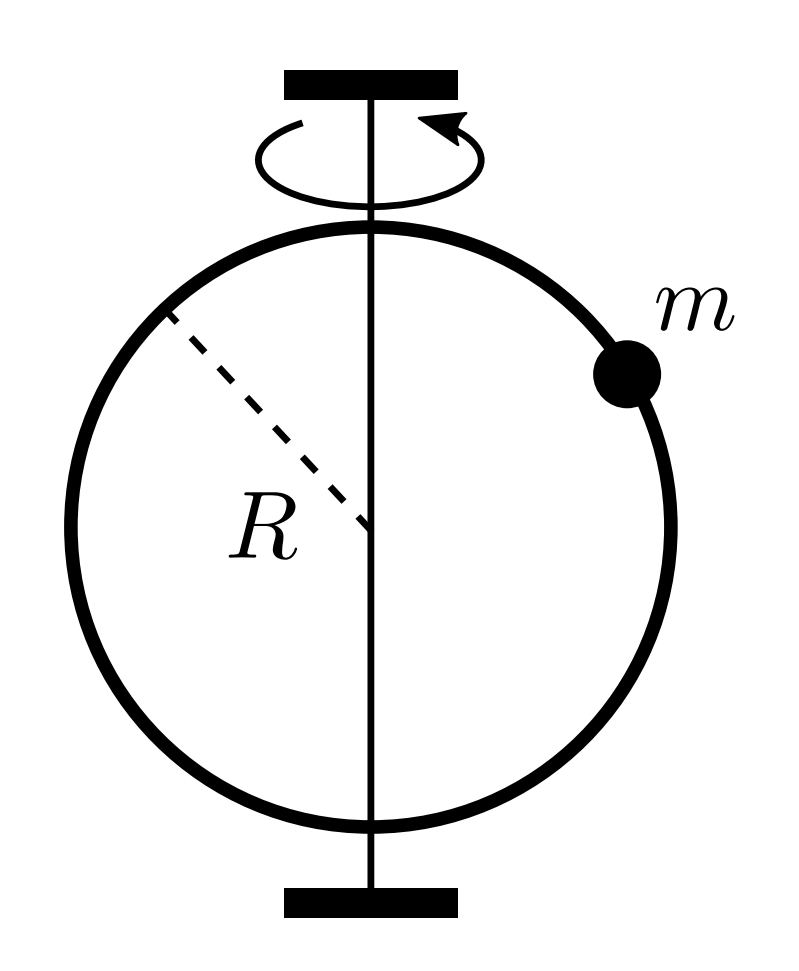
\includegraphics[width=0.2\textwidth]{content/Figures/4-6}
	\caption{ }
	\label{fig:4-6}
\end{figure}
	
\begin{solution}
    \begin{figure}[h]
    	\centering
    	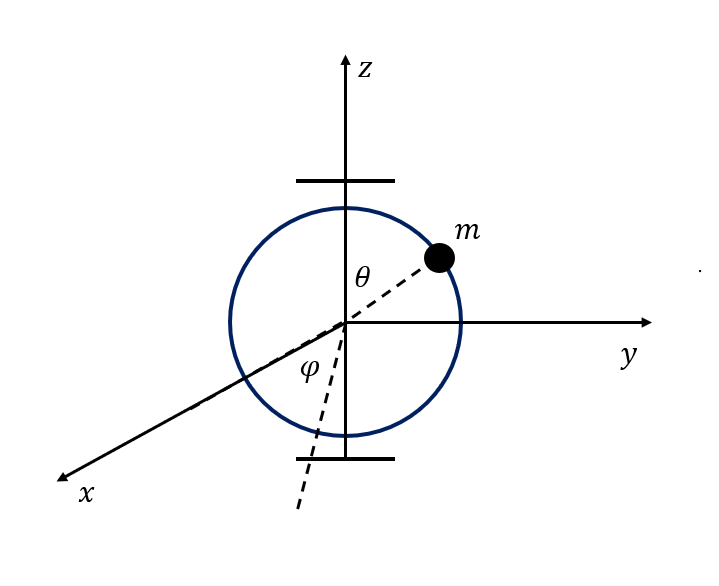
\includegraphics[width=0.4\textwidth]{content/Figures/4-6-1}
    	\caption{ }
    	\label{fig:4-6-1}
    \end{figure}
    如图\ref{fig:4-6-1}选取广义坐标。以圆环中心为坐标原点,那么可以写出\(m\)的坐标为
    \begin{align*}
    	x&=-R\sin{\theta}\sin{\varphi}\\
    	y&=R\sin{\theta}\cos{\varphi}\\
    	z&=R\cos{\theta}
    \end{align*}
    动能为\footnote{此处的详细计算过程请看附带的mathematica代码。}
    \begin{align*}
    	T&=\frac{1}{2}I \dot\varphi^2+\frac{1}{2}m(\dot{x}^2+\dot{y}^2+\dot{z}^2)\\
    	&=\frac{1}{2}(I+mR^2 \sin^2{\theta})\dot{\varphi}^2+\frac{1}{2}mR^2 \dot{\theta}^2
    \end{align*}
    而势能为
    \[V=mgz=mgR\cos{\theta}\]
    拉格朗日量为
    \[L=T-V=\frac{1}{2}(I+mR^2 \sin^2{\theta})\dot{\varphi}^2+\frac{1}{2}mR^2 \dot{\theta}^2-mgR\cos{\theta}\]
    代入欧拉-拉格朗日方程
    \begin{align*}
    	\frac{\partial L}{\partial \theta}-\frac{\dd}{\dd t}\frac{\partial L}{\partial \dot{\theta}}=0\\
    	\frac{\partial L}{\partial \varphi}-\frac{\dd}{\dd t}\frac{\partial L}{\partial \dot{\varphi}}=0
    \end{align*}
    得到运动方程为
    \begin{align*}
    	mgR \sin{\theta}-m R^2 \ddot{\theta}+m R^2 \sin{\theta} \cos{\theta} \dot{\varphi}^2=0\\
    	-\left(I+m R^2 \sin^2{\theta}\right)\ddot{\varphi} -2 m R^2 \sin{\theta} \cos{\theta}\dot{\varphi}\dot{\theta}=0
    \end{align*}
\end{solution}


\problem{已知拉格朗日量在广义坐标的变换\(q^a\to \tilde{q}^a\)下不变,即有\(\tilde{L}(t,\tilde{q},\dot{\tilde{q}})=L(t,q,\dot{q})\)。(1)
	利用广义速度的变换(2.13),根据广义动量的定义\(p_a=\frac{\partial L}{\partial \dot{q}^a}\)和\(\tilde{p}_a=\frac{\partial L}{\partial \dot{\tilde{q}}^a}\),证明广义动量的变换为\(\tilde{p}_a=\frac{\partial q^b}{\partial \tilde{q}^a}p_b\);(2)在平面极坐标下写出非相对论性自由粒子的拉格朗日量,并求\(\{p_x, p_y\}\)和\(\{p_r, p_\phi\}\)的关系,以验证(1)的结论。}

\begin{solution}
    (1)首先将书上(2.13)抄于此处
    \[\frac{\partial\dot{\tilde{q}}^a}{\partial\dot{q}^b}=\frac{\partial\tilde{q}^a}{\partial\tilde{q}^b},\frac{\partial \dot{q}^a}{\partial \dot{\tilde{q}}^b}=\frac{\partial q^a}{\partial \tilde{q}^b}\]
    接下来进行证明。只需计算
    \[\tilde{p}_a=\frac{\partial L}{\partial \dot{\tilde{q}}^a}=\frac{\partial L}{\partial \dot{q}^b}\frac{\partial \dot{q}^b }{\partial \dot{\tilde{q}}^a}=\frac{\partial q^b}{\partial \tilde{q}^a}\frac{\partial L}{\partial \dot{q}^b}=\frac{\partial q^b}{\partial \tilde{q}^a} p_b\]
    证毕。
    
    (2)平面极坐标系自由粒子的拉格朗日量应当记得为
    \[L=\frac{1}{2}m(\dot{r}^2+r^2\dot{\phi}^2)\]
    极坐标系与直角坐标系的关系为
    \begin{align*}
    	x=r\cos{\phi}\\
    	y=r\sin{\phi}
    \end{align*}
    那么可以算出
    \[p_r=\frac{\partial L}{\partial \dot{r}}=m\dot{r}=m\frac{x\dot{x}+y\dot{y}}{\sqrt{x^2+y^2}}=\frac{x p_x+y p_y}{\sqrt{x^2+y^2}}\]
    \[p_\phi=\frac{\partial L}{\partial \dot{\phi}}=mr^2\dot{\phi}=m(x\dot{y}-y\dot{x})=x p_y-y p_x\]
    如果直接代入公式,那么结果为
    \[p_r=\frac{\partial x}{\partial r}p_x+\frac{\partial y}{\partial r}p_y=\cos{\phi}p_x+\sin{\phi}p_y=\frac{x p_x+y p_y}{\sqrt{x^2+y^2}}\]
    \[p_\phi=\frac{\partial x}{\partial \phi}p_x+\frac{\partial y}{\partial \phi}p_y=-r\sin{\phi}p_x+r\cos{\phi}p_y=-y p_x+x p_y\]
    验证完毕。
\end{solution}


\problem{}
\begin{solution}
    待施工.
\end{solution}



\problem{}
\begin{solution}
    待施工.
\end{solution}



\problem{}
\begin{solution}
    待施工.
\end{solution}



\problem{考虑与标量场相互作用的粒子作用量的 4 维形式和 3 维形式, 分别求粒子运动方程的 4 维形式和 3 维形式.}
\begin{solution}
    Minkowski 时空标量场中的粒子,其作用量为
    \[
        S = - m c \int \dd \tau \,\me^{\Phi} \sqrt{- \eta_{\mu \nu} \frac{\dd x^\mu}{\dd \tau} \frac{\dd x^\nu}{\dd \tau}},
    \]
    将被固有时 $\tau$ 参数化后的世界线 (作用量) 对 $x^\mu$ 作变分:
    \begin{align*}
        \delta S &= - mc \int \dd \tau \left[\frac{\pp}{\pp x^\mu} \left(\me^{\Phi} \sqrt{- \eta_{\mu \nu} \frac{\dd x^\mu}{\dd \tau} \frac{\dd x^\nu}{\dd \tau}}\right) \delta x^\mu + \frac{\pp}{\pp \left(\frac{\dd x^\mu}{\dd \tau}\right)} \left(\me^{\Phi} \sqrt{- \eta_{\mu \nu} \frac{\dd x^\mu}{\dd \tau} \frac{\dd x^\nu}{\dd \tau}}\right)\delta \left(\frac{\dd x^\mu}{\dd \tau}\right)\right]  \\
        &= - mc \int \dd \tau \left[\frac{\pp \Phi}{\pp x^\mu} \me^{\Phi} \sqrt{- \eta_{\mu \nu} \frac{\dd x^\mu}{\dd \tau} \frac{\dd x^\nu}{\dd \tau}} \delta x^\mu - \me^{\Phi} \frac{\eta_{\mu \nu} \frac{\dd x^\nu}{\dd \tau}}{\sqrt{- \eta_{\mu \nu} \frac{\dd x^\mu}{\dd \tau} \frac{\dd x^\nu}{\dd \tau}}} \delta \left(\frac{\dd x^\mu}{\dd \tau}\right)\right] \\
        & \simeq -mc \int \dd \tau \left[\frac{\pp \Phi}{\pp x^\mu} \me^{\Phi} \sqrt{- \eta_{\mu \nu} \frac{\dd x^\mu}{\dd \tau} \frac{\dd x^\nu}{\dd \tau}} + \frac{\dd}{\dd \tau} \left(\me^{\Phi} \frac{\eta_{\mu \nu} \frac{\dd x^\nu}{\dd \tau}}{\sqrt{- \eta_{\mu \nu} \frac{\dd x^\mu}{\dd \tau} \frac{\dd x^\nu}{\dd \tau}}}\right) \right] \delta x^\mu,
    \end{align*}
    因为 4-速度的模方是常数 $\eta_{\mu \nu} \frac{\dd x^\mu}{\dd \tau} \frac{\dd x^\nu}{\dd \tau} = - c^2$, 且由度规升降 $\eta_{\mu \nu} \frac{\dd x^\nu}{\dd \tau} \equiv \frac{\dd x_\mu}{\dd \tau}$, 所以我们可以写出 Euler-Lagrange 方程:
    \begin{align*}
        - \frac{1}{mc} \frac{\delta S}{\delta x^\mu} &= \frac{\pp \Phi}{\pp x^\mu} \me^\Phi c + \frac{\dd}{\dd \tau} \left(\frac{\me^\Phi}{c} \frac{\dd x_\mu}{\dd \tau}\right) = 0 \\
        &= c \frac{\pp \Phi}{\pp x^\mu} \me^\Phi + \frac{1}{c} \frac{\dd x_\mu}{\dd \tau} \frac{\pp \me^\Phi}{\pp \tau} + \frac{\me^\Phi}{c} \frac{\dd^2 x_\mu}{\dd \tau^2} = 0 \\
        &= c \frac{\pp \Phi}{\pp x^\mu} \me^\Phi + \frac{1}{c} \frac{\dd x_\mu}{\dd \tau} \frac{\pp x^\nu}{\pp \tau} \frac{\pp \Phi (x^\mu)}{\pp x^\nu} \me^\Phi + \frac{\me^\Phi}{c} \frac{\dd^2 x_\mu}{\dd \tau^2} = 0,
    \end{align*}
    即 4 维形式的运动方程
    \[
        \frac{\dd^2 x_\mu}{\dd \tau^2} + \frac{\pp \Phi}{\pp x^\nu} \frac{\pp x^\nu}{\pp \tau} \frac{\dd x_\mu}{\dd \tau} + c^2 \frac{\pp \Phi}{\pp x^\mu} = 0, \quad \mu = 0, 1, 2, 3.
    \]
    标量场作用下的作用量的 3 维形式为
    \[
        S = - m c \int \dd t\,\me^\Phi \sqrt{1- \frac{\delta_{ij}}{c^2} \frac{\dd x^i}{\dd t} \frac{\dd x^j}{\dd t}},
    \]
    对 3 维坐标 $x^i$ 作变分:
    \begin{align*}
        \delta S &= - mc \int \dd t \left[\frac{\pp}{\pp x^i} \left(\me^\Phi \sqrt{1- \frac{\delta_{ij}}{c^2} \frac{\dd x^i}{\dd t} \frac{\dd x^j}{\dd t}}\right) \delta x^i + \frac{\pp}{\pp \left(\frac{\dd x^i}{\dd t}\right)} \left(\me^\Phi \sqrt{1- \frac{\delta_{ij}}{c^2} \frac{\dd x^i}{\dd t} \frac{\dd x^j}{\dd t}}\right) \delta \left(\frac{\dd x^i}{\dd t}\right)\right] \\
        &= - mc \int \dd t \left[\frac{\pp \Phi}{\pp x^i} \me^\Phi \sqrt{1- \frac{\delta_{ij}}{c^2} \frac{\dd x^i}{\dd t} \frac{\dd x^j}{\dd t}} \delta x^i - \me^\Phi \frac{\delta_{ij} \frac{\dd x^j}{\dd t} \delta \left(\frac{\dd x^i}{\dd t}\right)}{c^2 \sqrt{1- \frac{\delta_{ij}}{c^2} \frac{\dd x^i}{\dd t} \frac{\dd x^j}{\dd t}}}\right] \\
        & \simeq - mc \int \dd t \left[\frac{\pp \Phi}{\pp x^i} e^\Phi \sqrt{1 - \frac{\vec{v}^2}{c^2}} + \frac{\dd}{\dd t} \left(\frac{\me^\Phi}{c^2} \frac{\frac{\dd x_i}{\dd t}}{\sqrt{1 - \frac{\vec{v}^2}{c^2}}}\right)\right] \delta  x^i, \\
        - \frac{\delta S}{\delta x^i} &= m c \frac{\pp \Phi}{\pp x^i} \me^\Phi \sqrt{1 - \frac{\vec{v}^2}{c^2}} + \frac{\me^\Phi}{c^2} \dot{\Phi} \frac{mc \frac{\dd x_i}{\dd t}}{\sqrt{1 - \frac{\vec{v}^2}{c^2}}} + \frac{\me^\Phi}{c^2} \frac{mc \frac{\dd^2 x_i}{\dd t^2}}{\sqrt{1 - \frac{\vec{v}^2}{c^2}}} = 0,
    \end{align*}
    3-动量定义为 $p_i \equiv m \frac{\dd x_i}{\dd t} \frac{\dd t}{\dd \tau} \equiv m \frac{\dd x_i}{\dd t} \frac{1}{\sqrt{1 - \frac{\vec{v}^2}{c^2}}}$, 则上式整理为, 
    \[
        \frac{\me^\Phi}{c} \left(\dot{\Phi} p_i + \dot{p}_i\right) + mc \frac{\pp \Phi}{\pp x^i} \me^\Phi \sqrt{1 - \frac{\vec{v}^2}{c^2}} = 0,
    \]
    即 3 维形式的运动方程
    \[
        \dot{p}_i + \dot{\Phi} p_i + mc^2 \sqrt{1 - \frac{\vec{v}^2}{c^2}} \frac{\pp \Phi}{\pp x^i} = 0, \quad i = 1, 2, 3.
    \]
\end{solution}



\problem{电磁场中带电粒子作用量的 4 维形式和 3 维形式分别为
    \begin{align*}
        S = \int \dd \tau L, \quad L = - m c \sqrt{- u_\mu u^\mu} + \frac{e}{c} A_\mu u^\mu, \\
        S = \int \dd \tau L, \quad L = - m c^2 \sqrt{1 - \frac{\vec{v}^2}{c^2}} - e \Phi + \frac{e}{c} \vec{v} \cdot \vec{A}.
    \end{align*}
    \begin{enumerate}[label=(\arabic*)]
        \item 求粒子的 4-共轭动量 $P_\mu \equiv \frac{\pp L}{\pp u^\mu}$ 和 3-共轭动量 $P_i \equiv \frac{\pp L}{\pp \dot{x}^i}$;
        \item 分别求粒子运动方程的 4 维形式和 3 维形式; 
        \item 若 $E$ 由式
        \[
            E := c p^0 = m c u^0 = m c^2 \frac{\dd t}{\dd \tau} = \frac{m c^2}{\sqrt{1 - \frac{\vec{v}^2}{c^2}}}
        \]
        给出, 证明 $\frac{\dd E}{\dd t} = e \vec{v} \cdot \vec{E}$.
    \end{enumerate}
}

\begin{solution}
    \begin{enumerate}[label=(\arabic*)]
        \item 待施工.
    \end{enumerate}
\end{solution}



\problem{由引力场中粒子的作用量(4.53)出发,证明粒子的运动方程为\(\frac{\dd u^\sigma}{\dd \tau}+{\Gamma^\sigma}_{\mu\nu}u^\mu u^\nu=0\),其中\(u^\mu\)为粒子的 4-速度,系数\({\Gamma^\sigma}_{\mu\nu}=\frac{1}{2}g^{\sigma\rho}(\frac{\partial g_{\rho\nu}}{\partial x^\mu}+\frac{\partial g_{\rho\mu}}{\partial x^\nu}-\frac{\partial g_{\mu\nu}}{\partial x^\rho})\)被称为列维-契维塔联络。}

\begin{solution}
	待施工.
\end{solution}



\problem{观察到某非相对论性自由粒子\(t = 0\)时刻处于\(x = 0\)处,\(t_*\)时刻处于\(x_*\)处。(1)考虑三种运动方式:匀速直线运动\(x(t)=x_* \frac{t}{t_*}\),匀加速运动\(x(t)=x_*\left(\frac{t}{t_*}\right)^2\)和谐振动\(x(t)=x_*\sin{\left(\frac{\pi}{2} \frac{t}{t_*}\right)}\),都满足端点条件,证明匀速直线运动对应的作用量数值最小;(2)考虑运动方式\(x(t)=x_*\left(\frac{t}{t_*}\right)^n\),也都满足端点条件,证明当\(n=1\)(即匀速直线运动)时,作用量取最小值。}

\begin{solution}
	(1)非相对论自由粒子拉格朗日量为\(L=T=\frac{1}{2}m \dot{x}^2\),于是其作用量可写为
	\[S=\int_{0}^{t_*}\frac{1}{2}m \dot{x}(t)^2 \dd t\]
	代入不同的\(x(t)\)计算数值即可,结果为\footnote{计算过程见mathematica代码。}:
	\begin{align*}
		S=\begin{cases}
			\frac{m x_*^2}{2 t_*},  x(t)=x_* \frac{t}{t_*}\\
			\frac{2 m x_*^2}{3 t_*}, x(t)=x_*\left(\frac{t}{t_*}\right)^2\\
			\frac{\pi ^2 m x_*^2}{16 t_*}, x(t)=x_*\sin{\left(\frac{\pi}{2} \frac{t}{t_*}\right)}
		\end{cases}
	\end{align*}
	对比系数可知匀速运动的作用量数值最小。
	
	(2)\(x(t)=x_*\left(\frac{t}{t_*}\right)^n\),代入计算出作用量为
	\[S=\int_{0}^{t_*}\frac{1}{2}m \dot{x}(t)^2 \dd t=\frac{n^2}{4n-2}\frac{m x_*^2}{t_*}\]
	求导可知
	\[\frac{\partial S}{\partial n}=\frac{(n-1) n}{(2n-1)^2}\frac{m x_*^2}{t_*}\]
	最小值点为\(n=1\),为匀速直线运动,证毕。
\end{solution}



\problem{取竖直向上为\(z\),已知自由落体小球的拉格朗日量为\(L=\frac{1}{2}m\dot{z}^2-mgz\),假设小球在\(t_1\)时刻处在\(z_1\),在\(t_2\)时刻处在\(z_2\)。(1)求\(z(t)\)的运动方程,并求满足上述端点条件的定解\(z_{cl}(t)\);( 2)求此定解\(z_{cl} (t)\)对应的作用量的数值\(S_{cl}\);(3)相对于其他非真实的运动,验证\(Scl\)是最小还是最大?(提示,令\(z(t)=z_{cl}(t)+\epsilon \delta z(t)\),有\(S-S_{cl}=\epsilon \delta S+\frac{\epsilon^2}{2}\delta^2 S+\cdots\)。因为\(\delta S=0\),所以即需要验证二阶变分\(\delta^2 S\)是正的还是负的。)}

\begin{solution}
	(1)由欧拉-拉格朗日方程
	\[\frac{\partial L}{\partial z}-\frac{\dd}{\dd t}\frac{\partial L}{\partial \dot{z}}=0\]
	得到运动方程为
	\[-mg-m\ddot{z}=0\]
	即\(\ddot{z}=g\),\(z(t)=a+bt+\frac{1}{2}gt^2\),结合初始条件,得到
	\begin{align*}
		a&=-\frac{-g t_1^2 t_2+g t_1 t_2^2-2 t_1 z_2+2 t_2 z_1}{2 (t_1-t_2)}\\
		b&=-\frac{g t_1^2-g t_2^2-2 z_1+2 z_2}{2 (t_1-t_2)}
	\end{align*}
	也就是说
	\[z_{cl}(t)=-\frac{-g t_1^2 t_2+g t_1 t_2^2-2 t_1 z_2+2 t_2 z_1}{2 (t_1-t_2)}-\frac{g t_1^2-g t_2^2-2 z_1+2 z_2}{2 (t_1-t_2)}t+\frac{1}{2}g t^2\]
	
	(2)作用量为\footnote{以下计算使用mathematica。}
	\begin{align*}
		S_{cl}&=\int_{t_1}^{t_2} L(z_{cl}(t),\dot{z}_{cl}(t),t)\dd t\\
		&=\int_{t_1}^{t_2} \left(\frac{1}{2}m\dot{z}_{cl}(t)^2-mgz_{cl}(t) \right)\dd t\\
		&=\frac{1}{8} m (t_2-t_1) \left(g^2 (t_2-t_1)^2-4 g (z_1+z_2)+\frac{4 (z_2-z_1)^2}{(t_2-t_1)^2}\right)
	\end{align*}
	
	(3)考虑对作用量进行变分,即
	\begin{align*}
		S[z_{cl}+\epsilon \delta z]-S[z_{cl}]&=\int_{t_1}^{t_2} \left[L(z_{cl}+\epsilon \delta z,\dot{z}_{cl}+\epsilon \delta \dot{z},t)-L(z_{cl},\dot{z}_{cl},t)\right]\dd t\\
		&=\int_{t_1}^{t_2}\left[\frac{1}{2}m(\dot{z}_{cl}+\epsilon \delta \dot{z})^2-mg(z_{cl}+\epsilon \delta z)-(\frac{1}{2}m\dot{z}_{cl}^2-mgz_{cl})\right]\dd t\\
		&=\int_{t_1}^{t_2}\left[\epsilon m\dot{z}_{cl}\delta \dot{z}-\epsilon mg \delta z+\epsilon^2\frac{1}{2}m \delta \dot{z}^2 \right]\dd t\\
		&=\epsilon m \dot{z}\delta z(t)\bigg|_{t_1}^{t_2}+\epsilon\int_{t_1}^{t_2} \left[-m\ddot{z}_{cl}-mg\right]\dd t+\epsilon^2\int_{t_1}^{t_2}\frac{1}{2}m \delta \dot{z}^2 \dd t\\
		&=\epsilon^2\int_{t_1}^{t_2}\frac{1}{2}m \delta \dot{z}^2 \dd t\\
		&\geq 0
	\end{align*}
	因此\(S_{cl}\)为最小作用量。
\end{solution}



\problem{}
\begin{solution}
	待施工.
\end{solution}



\problem{}
\begin{solution}
	待施工.
\end{solution}


